\chapter{Results and Analysis}

\section{Throughput vs Node Placement and Mobility}

As stated in previous chapter, we performs three simulations with different types of mobility, namely static circular location, static random distribution within a disc, and dynamic 2D random walk. The result from simulation scenario throughput vs node placement and mobility can be seen in Figure~\ref{fig:result-mobility-combine}. 

\begin{figure}[H]
    \centering
    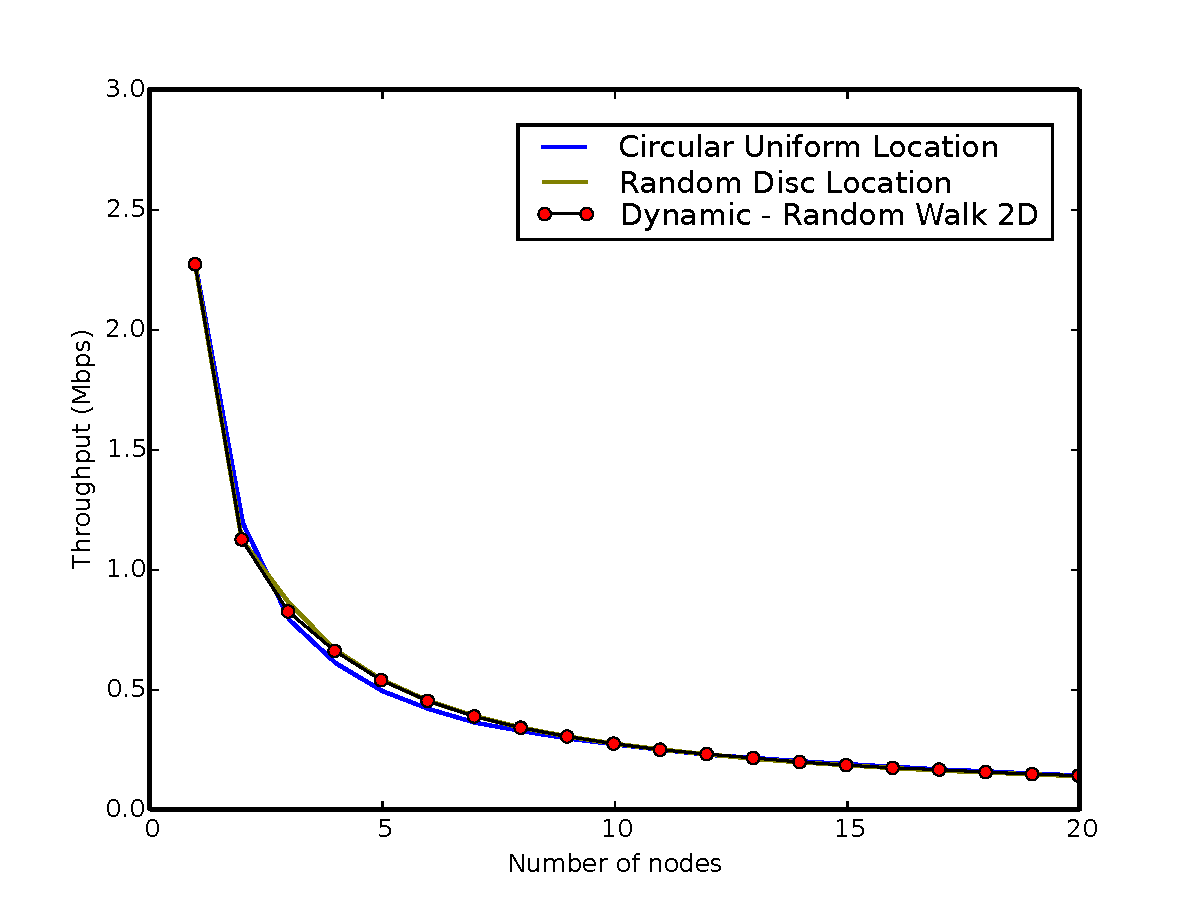
\includegraphics[width=0.8\textwidth]{figures/result-mobility-combine}
    \caption{Average throughput on different types of mobility}
    \label{fig:result-mobility-combine}
\end{figure}

From Figure~\ref{fig:result-mobility-combine}, it is obvious that for all modes, the average throughput goes down as the number of nodes incerases. However, there are only slight differences among them. Thus, we need additional information in order to get the valuable results. The value of standard deviation from each of simulations can be used as a solution. Figure~\ref{fig:std-combine} depicts the standard deviation for three different modes of node mobility.

We can see from Figure~\ref{fig:std-combine} that the static circular placement of nodes gives low standard deviation for the total number of nodes below 10 whereas above 10, the standard deviation values are quite similar with the other modes. This is because for a small number of nodes, the circular placement is distributed uniformly so that the distance between AP and nodes are equal.

\begin{figure}[H]
    \centering
    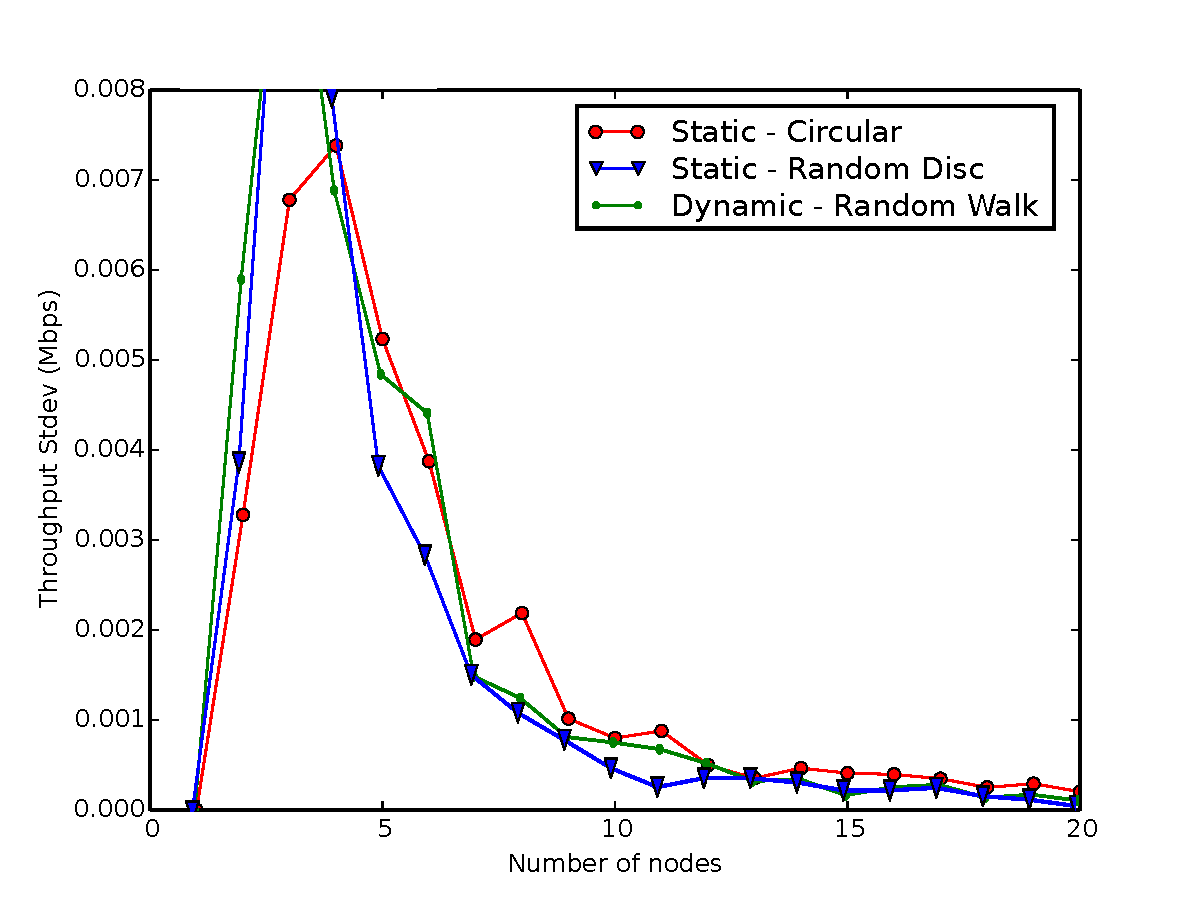
\includegraphics[width=0.8\textwidth]{figures/std-combine}
    \caption{Standard deviation of throughput on different types of mobility}
    \label{fig:std-combine}
\end{figure}

\section{Throughput vs Payload Size}

Figure~\ref{fig:payloads} depicts the effect of payload size to the average throughput of the system.

\begin{figure}[H]
    \centering
    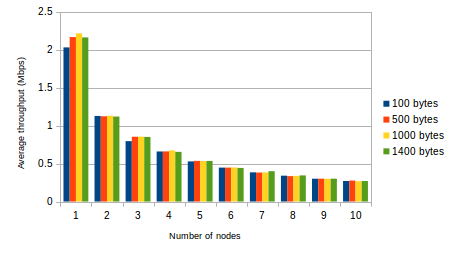
\includegraphics[width=0.8\textwidth]{figures/payloads}
    \caption{Throughput with and without using RTS/CTS}
    \label{fig:payloads}
\end{figure}

We can see from Figure~\ref{fig:payloads} that for small number of nodes, the throughput is lower when we use 100 bytes as payloads. For large number of nodes, the higest payload gives the better results. This happen because when the payload size is decreased, the transmitted bytes (Tx) will also decrease, reducing the number of received bytes (Rx). Thus, as throughput depends on Rx bytes and the simulation time is made constant, the throughput is decreasing. To tacke this problem, we can use the maximum value of payload size.

\section{Throughput vs The Use of RTS/CTS}

Figure~\ref{fig:rts-cts-combine} shows the effect of RTS/CTS that reduces the throughput. This happens because RTS/CTS adds more overhead to the system, hence lowering the throughput.

\begin{figure}[H]
    \centering
    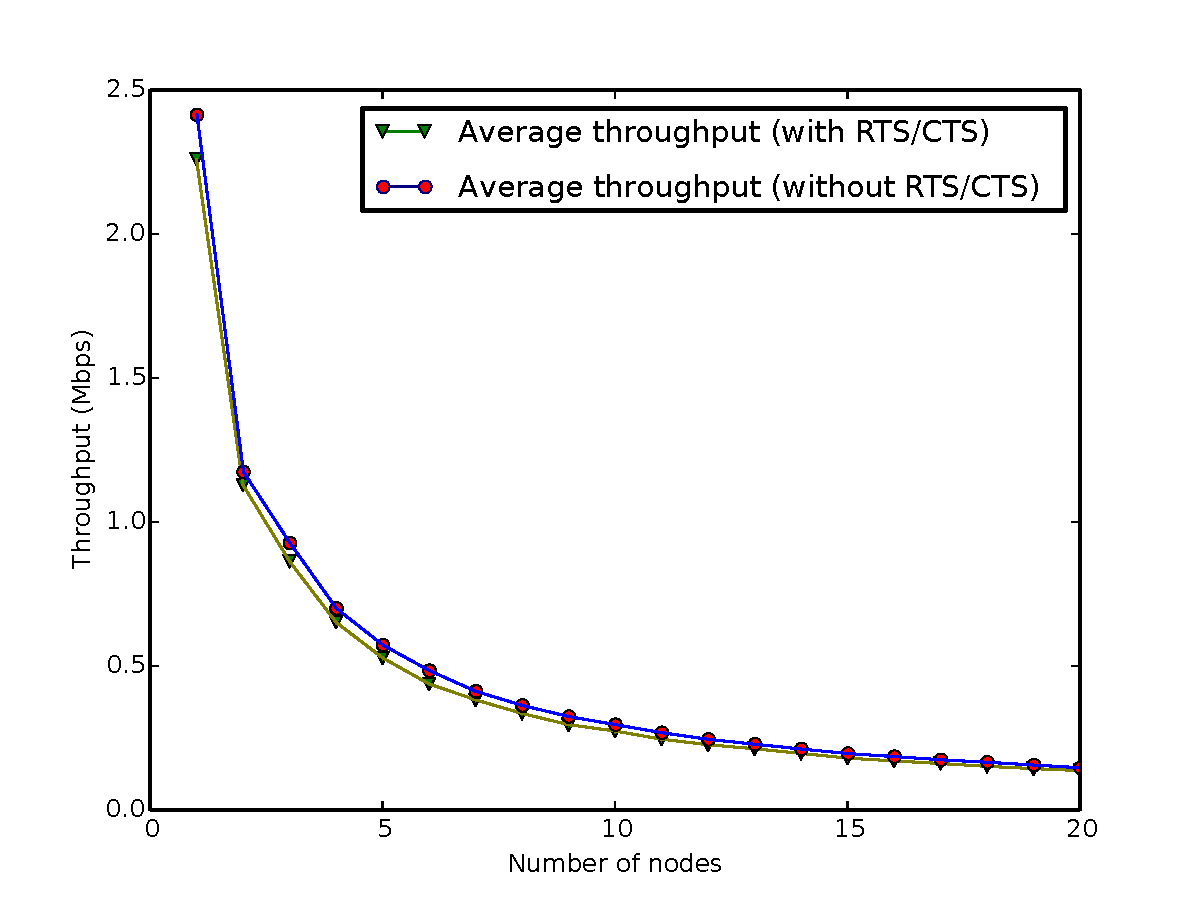
\includegraphics[width=0.8\textwidth]{figures/rts-cts-combine}
    \caption{Throughput with and without using RTS/CTS}
    \label{fig:rts-cts-combine}
\end{figure}

Basically, the use of RTS/CTS can increase the throughput. However, in this simulation, the throughput is lower than expected. There are two reasons that probably triggers this problem. First, TCP has three-way of handshaking mechanism to reduce collision. Thus, RTS/CTS does not give a big impact on the average of throughput for a system with a large number of nodes. Secondly, since only one AP is used in this simulation and such AP covers all of the nodes in the system, there is no hidden problem occurs. Also, the exposed node problem does not exist. Therefore, RTS/CTS does not give any advantage to the increasing number of throughput.